\documentclass[main.tex]{subfiles}
\begin{document}
\onlyinsubfile{\mainmatter{}}

\chapter{Background: Ensuring Memory Safety using Capabilities} \label{ch:cheri}
Most security bugs classified as \enquote{serious} in large projects such as the Chromium browser engine are memory safety bugs \citep{chromium} — bugs such as out-of-bounds array or call stack accesses that arise from the use of \enquote{memory-unsafe} programming languages like C, the use of memory safety opt-outs (such as Rust’s \texttt{unsafe}) in \enquote{memory-safe} programming languages, bugs in the compiler, bugs in the standard library implementation of a memory-safe programming language, or bugs in the runtime environment such as the Java VM or an ECMAScript interpreter.

Common approaches to mitigating attacks or restricting the attack vector that such a bug can cause include reintroducing compiler-inserted array bounds checks in memory-unsafe programming languages and enforcing page-level permissions in the virtual memory system of the operating system. However, runtime checks introduce a runtime cost, and virtual memory protection doesn’t protect against a compromised or vulnerable library such as Apache Log4j accessing potentially sensitive data in the process’ address space such as TLS session keys stored in an in-process OpenSSL data structure.

A different approach are \textbf{capabilities}, which are unforgeable tokens that carry authority over an entity.\citep[Section~1.1]{capsys} They have been described (without naming them) since at least the 1970s, e.g., in the context of the Multics timesharing system (which later played an important role in the design of Unix) by \citet{multics}, but renewed research interest has emerged since the development of a design for a new capability machine called CHERI in the early 2010s,\citep[Section~A.1, Chapter~13]{cheri} which we discuss in the next section.

In this thesis, capabilities are unforgeable pointers that carry authority over a precise region of memory for a specified set of operations. While virtual memory systems provide coarse-grained memory protection, usually at the level of a page, capabilities provide \emph{fine-grained} memory protection. A memory allocator can for instance return a capability that grants access to (and only to) the allocated region of memory. To ensure that authority cannot be created, capabilities can only be derived from a source with more authority, such as an operating system, a more privileged routine, or another capability. Finally, capability support can be provided at the hardware level, removing the runtime cost associated with software-based bounds \& permission checks.

\section{Capability Hardware Enhanced RISC Instructions}
\textbf{CHERI} (\textbf{Capability Hardware Enhanced RISC Instructions}; see also \citet{intro2cheri}) is a design for a capability machine, extending several existing instruction set architectures (ISAs) such as RISC-V, MIPS, x86-64, and Arm with hardware capability support. One of CHERI’s design goals is to provide a viable transition path for mainstream systems. An ecosystem formed around CHERI, such as capability extensions for C \& C++, capability support in the LLVM compiler toolchain and QEMU emulator, a FreeBSD fork with capability support called CheriBSD, and several large libraries and systems such as PostgreSQL and WebKit being ported to CheriBSD. Additionally, CHERI supports an execution mode that allows capability-unaware code to work as if they're executed on non-capability hardware.\footnote{CHERI also supports a hybrid model where compilers can implement return addresses and function pointers using capabilities while implementing other pointers using capability-unaware instructions, thereby improving the security of legacy code without breaking it. Capability-unaware instructions in CHERI-RISC-V evaluate pointers as offsets of the capability in the DDC (Default Data Capability) register, which a capability-aware operating system or runtime can configure before passing control to the capability-unaware program.}

In 64-bit CHERI-RISC-V, the CHERI extension of the 64-bit RISC-V ISA, 64-bit pointers become 128-bit capabilities. As illustrated in \cref{fig:chericoncentrate}, such a capability consists of a 64-bit address, a 27-bit compressed value indicating the capability’s bounds relative to the address, a 16-bit permissions mask (specifying permissions such as \emph{permit load}), with the remaining 21 bits reserved for encoding other flags and the capability’s object type (used for a CHERI feature called \enquote{\gls*{sealing}}, cf. infra). A 1-bit validity tag is set when the 128-bit datum represents a valid capability; this bit cannot be set in software.\footnote{The processor sets internally a validity bit for each register that holds a capability. For capabilities in memory, validity tags are stored out-of-band in tagged memory for each capability-aligned memory location. This also implies that capabilities can only be stored in capability-aligned memory locations.} The tag is cleared whenever the capability is modified by any instruction such as \texttt{XOR} or \texttt{ADD} not intended to modify capabilities.

CHERI-RISC-V defines several capability-aware instructions that \emph{can} modify capabilities via guarded manipulation. For instance, \texttt{CAndPerm} removes permissions from a given capability by performing a bitwise conjunction with a given permissions mask whereas \texttt{CIncOffset} adds an offset to a given capability's address. These limitations are in place to ensure 4 important safety properties of capability machines and CHERI architectures in particular, briefly summarised here below.

\begin{figure}
	\centering
	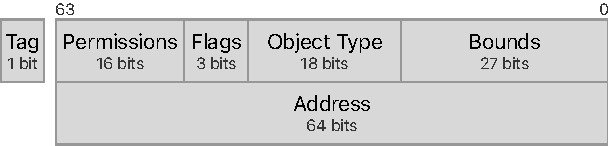
\includegraphics{Images/CHERI Concentrate Layout.pdf}
	\caption{A simplified layout of a 256-bit CHERI capability compressed into 128 bits using the CHERI Concentrate encoding. CHERI-RISC-V defines one flag bit and reserves the other two bits for future use. The validity tag bit is stored out-of-band, usually in tagged memory not directly accessible by user programs.}
	\label{fig:chericoncentrate}
\end{figure}

\paragraph{Permissions} A capability specifies zero or more permissions that the holder of the capability is allowed to exercise. For example, the \emph{permit load} resp. \emph{permit store} permissions allow the holder to load resp. store data in the region of memory specified by the capability. Beyond permissions also found in traditional virtual memory systems, capabilities also support CHERI-specific permissions such as \emph{permit capability load} and \emph{permit capability store}. Performing an action not allowed by the capability, such as storing data using a load-only capability, results in a machine trap.\footnote{In some specific cases, such as loading a capability using a capability that only allows loading data but not capabilities, merely results in a capability's tag being cleared, thereby deactivating any authority that it otherwise might unintentionally have conferred.}

\paragraph{Bounds} A capability specifies a contiguous region of memory where the holder of the capability is allowed exercise actions permitted by the capability's permissions. For example, a capability produced by a secure, capability-aware implementation of \texttt{malloc} pointing to a heap-allocated buffer would only permit accesses within that buffer. Performing an action outside of these bounds, i.e., a buffer overflow, results in a machine trap.

\paragraph{Provenance} A capability can only be derived from other capabilities. Authority cannot be forged by modifying its in-memory representation; attempting to do so causes the capability's tag bit to be cleared which invalidates the capability. Tag bits cannot be set in software.

\paragraph{Monotonicity} A capability cannot have more authority than the capability it's derived from: permissions can only be removed and bounds can only be shrunk. At CPU reset, the hardware provides root capabilities to the bootloader or firmware, which can be iteratively restricted in higher levels of abstraction, as illustrated in \cref{fig:derivingauth}.

\begin{figure}
	\centering
	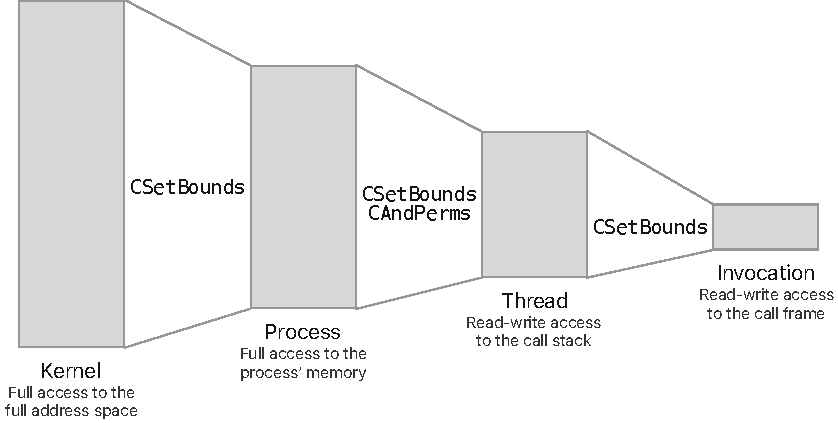
\includegraphics{Images/Deriving Authority.pdf}
	\caption{Provenance and monotonicity in action in protecting process memory, the call stack, and a call frame. The size of the depicted memory regions are not to scale. Similar illustrations can be made about a process' heap and heap-allocated memory.}
	\label{fig:derivingauth}
\end{figure}

\section{Sealed Capabilities}
CHERI provides a capability protection mechanism called \textbf{\g{sealing}}, whereby the capability holder is restricted from modifying or dereferencing the capability. The inverse operation, i.e., \textbf{\g{unsealing}}, is only allowed under specific circumstances. \G{sealing} comes in two forms: \g{sealing} using a \g{sealcap} or \g{sealing} as a \g{sentry}. The sealed state of a capability is encoded in its \textbf{\g{otype}} field; the \g{otype} of an unsealed capability has the special value $-1$.

\paragraph{Sealing using a seal capability} A capability with the \emph{permit seal} permission, i.e., a \textbf{\g{sealcap}}, can be used to seal another capability. The \g{otype} of the sealed capability is set to the \g{sealcap}'s \enquote{address}.\footnote{This \enquote{address} doesn't necessarily need to refer to a valid location in memory. A capability whose address is only used for sealing and unsealing capabilities should therefore omit the \emph{permit load} and \emph{permit store} family of permissions to avoid letting holders of the seal capability access invalid memory locations. Also note that the \g{otype} field is 18 bits wide whereas the address field is 64 bits wide: sealing with a \g{sealcap} whose address doesn't fit in 18 bits results in a machine trap. Additionally, \gs{otype} reserved by the architecture cannot be used for (un)sealing using a \g{sealcap}.} A capability with the \emph{permit unseal} permission, i.e., an \textbf{\g{unsealcap}}, can be used to unseal a sealed capability provided that the sealed capability's \g{otype} is equal to the \g{unsealcap}'s \enquote{address}. A \g{sealcap} can also act as an \g{unsealcap} if it has both permissions.

As would be expected from normal pointer-like capabilities, the (un)seal capability's address must be within its bounds when (un)sealing; otherwise a machine trap ensues. By carefully controlling access to and bounding capabilities with the \emph{permit seal} and \emph{permit unseal} permissions, sealing can be used for higher-level features such as encapsulation.

Sealing and unsealing can be done using the \texttt{CSeal} respectively \texttt{CUnseal} instructions. CHERI-RISC-V additionally provides a \texttt{CInvoke} instruction that takes a code and data capability pair with matching \g{otype}, unseals them, and jumps to the code capability's address. This feature enables secure domain transitions, wherein the caller cannot dereference the code or data capability (which may belong to a closure, for example), but can use them to perform an invocation.

\paragraph{Sealing as a sentry capability} An executable capability can be sealed by itself as a \textbf{\g{sentry}} using the \texttt{CSealEntry} instruction. CHERI-RISC-V defines a \texttt{CJALR} instruction that jumps to the address of a given target capability, unsealing the capability if it is a \g{sentry}. Similar to RISC-V's \texttt{JALR} instruction, the instruction also accepts a link register wherein it puts the return address. Unlike \texttt{JALR} however, \texttt{CJALR} also seals the \g{retcap} as a \g{sentry}, ensuring that the callee can only use it to return to the caller. A \g{sentry}'s \g{otype} has the special value $-2$.

\biblio{}
\onlyinsubfile{\glsaddall\printglossaries}
\end{document}
